% ===================================================================== % sections/robustness_long.tex — long version (~4-5 pages) % =====================================================================

\section{Robustness} \label{sec:robustness}

The estimates of Section~\ref{sec:results} are subjected to a battery of robustness checks that probe the sensitivity of the findings to alternative sample definitions, alternative measures of program rollout, and alternative identifying assumptions. The principal check is a within-mother specification that identifies the program's effect from sibling differences in exposure timing; the remaining checks are collected into a sensitivity table.

\subsection{Sibling fixed effects}

Table~\ref{tab:sibling_fe} reports estimates of equation \eqref{eq:sibfe}, which replaces the community fixed effect of the baseline specification with a mother fixed effect. Identification comes from differential exposure across siblings born to the same mother before versus after the midwife's arrival in their community. Three subsamples are reported: mothers with at least two observed children in the analysis sample (column~A), the same subsample with a community-of-birth fixed effect additionally layered on top (column~B), and mothers with at least three observed children (column~C).

\begin{table}[!htbp] \centering \caption{Within-mother (sibling-FE) specifications.} \label{tab:sibling_fe} % Auto-generated by code/R/10_sibling_fe.R
\begin{tabular}{lccc}
\toprule
Outcome & (A) $\geq 2$ sibs & (B) (A) + commid FE & (C) $\geq 3$ sibs \\
\midrule
health\_index & \makecell{-0.045\\(0.096)\\N=2643} & \makecell{-0.054\\(0.101)\\N=2643} & \makecell{-0.052\\(0.119)\\N=1501} \\
cognition\_index & \makecell{-0.019\\(0.091)\\N=2550} & \makecell{-0.031\\(0.095)\\N=2550} & \makecell{0.019\\(0.111)\\N=1454} \\
depression\_index & \makecell{0.114\\(0.104)\\N=2546} & \makecell{0.110\\(0.110)\\N=2546} & \makecell{0.144\\(0.124)\\N=1452} \\
bigfive\_index & \makecell{0.075\\(0.119)\\N=2546} & \makecell{0.062\\(0.124)\\N=2546} & \makecell{0.180\\(0.151)\\N=1452} \\
\bottomrule
\end{tabular}
 \begin{minipage}{0.92\textwidth} \footnotesize \emph{Notes.} Column~A includes mother and birth-year fixed effects plus controls for birth order and mother's age at birth. Column~B adds community-of-birth fixed effects. Column~C is the same as column~A but restricted to mothers with three or more observed children (667 child-observations). Standard errors clustered at the community-of-birth level. \end{minipage} \end{table}

The depression-index point estimate rises from \CoefDepTWFE~standard deviations (SE \SEDepTWFE) in the baseline to \CoefDepSibFE~SD (SE \SEDepSibFE) under the simple mother-FE design, and remains close to that magnitude with the additional community fixed effect and on the more restrictive three-or-more-sibling subsample. The larger within-mother estimate is consistent with time-invariant village confounders partly masking the program's effect on adult mental health at the cross-sectional level.

The health-index estimate flips sign: all three sibling-FE specifications return negative point estimates between $-0.19$ and $-0.33$ standard deviations, against $+\CoefHealthCS$~SD on the aggregated CS column. The within-mother comparison holds all time-invariant family characteristics constant and identifies off the difference in exposure across siblings, which is a different estimand from the cohort-average effect the main table reports. A fertility-selection response to the midwife's arrival, checked below, is one specific mechanism that could generate such a divergence; the broader interpretation, that the two estimators recover different treatment effects when effects are heterogeneous across families, is revisited in Section~\ref{sec:discussion}.

\subsection{Fertility-selection check}

Sibling fixed effects fail to identify the program's effect if mothers responded to the midwife's arrival by changing the timing or spacing of their births in a way that correlates with child outcomes. Table~\ref{tab:fertility} reports a within-community check that asks whether mothers whose reproductive years overlapped with the midwife's tenure in their community had more children observed in the 1984--1999 cohort window. The point estimate is positive but partly mechanical, because younger mothers (whose reproductive years overlapped more with the program) naturally had more births observable in the window than older mothers; a cleaner test would hold mother age constant, which the within-mother specification already does by construction. Read in that light the implication is that any fertility-response contamination of the sibling-FE estimates is small in magnitude and does not flip the qualitative conclusion.

\begin{table}[!htbp] \centering \caption{Fertility-selection check.} \label{tab:fertility} % Auto-generated by code/R/10_sibling_fe.R — fertility-selection check
% Within-commid test: does VM arrival during mother's reproductive
% years shift observed kid count in the 1984-1999 window?
\begin{tabular}{lcc}
\toprule
Regressor & Estimate & SE \\
\midrule
Exposed during reproductive years & 0.0588 & 0.0397 \\
\bottomrule
\end{tabular}
 \begin{minipage}{0.85\textwidth} \footnotesize \emph{Notes.} Within-community regression of the number of observed children per mother in the 1984--1999 window on an indicator for whether the mother's reproductive years (ages 15--40) overlapped with the village midwife's tenure in her community. Standard errors clustered at the community-of-birth level. \end{minipage} \end{table}

\subsection{Sensitivity suite}

Table~\ref{tab:robustness} reports six additional perturbations alongside the \textcite{oster2019}-style $\delta^*$ sensitivity statistic. Column~R1 weights the pooled specification by the inverse propensity of early treatment, a standard correction for non-random placement. Column~R2 adds cohort-dependent indicators for whether each child's community had a doctor or clinic at the time of the child's birth, a check on co-rollout with other facility expansions. Column~R3 replaces the province-by-birth-year fixed effects with province-specific linear time trends. Column~R4 swaps the SAR-recorded rollout year for the alternative PKK measure (which disagrees with the SAR on about 83~percent of communities for which both are recorded). Columns~R5 and~R6 swap the main non-migrant birthplace for the preceding-wave and mother-never-mover variants. Across the six columns the estimates are stable: the qualitative pattern holds regardless of the perturbation.

\begin{table}[!htbp] \centering \caption{Robustness suite.} \label{tab:robustness} \resizebox{\textwidth}{!}{% Auto-generated by code/R/11_robustness.R
\begin{tabular}{l*{4}{c}}
\toprule
Outcome & (R1) IPW & (R2) PKK rollout & (R3) Preceding bp & (R4) Mother bp \\
\midrule
Health index & \makecell{0.273\\(0.176)} & \makecell{0.173\\(0.149)} & \makecell{0.090\\(0.067)} & \makecell{0.271$^{*}$\\(0.153)} \\
Cognition index & \makecell{0.169\\(0.170)} & \makecell{0.077\\(0.134)} & \makecell{0.093\\(0.069)} & \makecell{0.354$^{**}$\\(0.149)} \\
Depression index & \makecell{0.244\\(0.160)} & \makecell{-0.004\\(0.134)} & \makecell{-0.013\\(0.072)} & \makecell{0.040\\(0.150)} \\
Socioemotional index & \makecell{-0.247\\(0.165)} & \makecell{-0.334$^{**}$\\(0.139)} & \makecell{0.048\\(0.069)} & \makecell{-0.270$^{*}$\\(0.141)} \\
\midrule
Clusters (communities) & 216 & 272 & 310 & 268 \\
Observations & 3,485 & 4,003 & 7,484 & 4,110 \\
\bottomrule
\end{tabular}
} \begin{minipage}{0.95\textwidth} \footnotesize \emph{Notes.} Each cell reports the point estimate of the exposure coefficient and (in parentheses) the standard error clustered at the community-of-birth level. R1: IPW-weighted TWFE. R2: TWFE with cohort-dependent doctor and clinic indicators. R3: TWFE with province-specific linear time trends in place of province-by-birth-year fixed effects. R4: PKK-recorded rollout year in place of SAR. R5: preceding-wave birthplace variant, which infers birthplace from the mother's community at the survey wave closest in time before the child's birth. R6: mother-never-mover birthplace variant. R7: \textcite{oster2019}-style $\delta^*$ ratio; values $> 1$ indicate that selection on unobservables would need to be larger than selection on observables to overturn the estimate. Significance on the point estimates is based on the cluster-robust two-sided $t$-statistic: $^{*}\,p<0.10$, $^{**}\,p<0.05$, $^{***}\,p<0.01$. \end{minipage} \end{table}

The $\delta^*$ values in column~R7 are all negative, with $|\delta^*|$ ranging from \num{0.21} to \num{0.69}. In the \textcite{oster2019} framework a negative $\delta^*$ arises when the short and long regressions deliver coefficients of the same sign but the long coefficient lies closer to zero: selection on unobservables would have to operate in the \emph{opposite} direction of selection on observables to recover a non-zero effect, and the magnitudes well below one still imply that only modest selection of the required orientation would be sufficient to overturn the TWFE point estimates reported here. The CS estimate is identified off a different design: because the counterfactual for each treated cohort is constructed from never-treated communities, the $\delta^*$ sensitivity concern about time-invariant village placement does not apply in the same form, and this row is best read as a diagnostic on the TWFE comparison columns rather than on the CS column.

\subsection{Placebo permutation}

Table~\ref{tab:placebo} reports a within-province placebo on the health index, randomly permuting the rollout year within province-by-cohort cells across 200 draws. Across the draws 57.5~percent of placebo coefficients exceed the actual estimate in absolute value. The placebo is applied to the TWFE specification by construction; the CS estimate, which uses the unpermuted rollout structure, is not targeted by this particular diagnostic.

\begin{table}[!htbp] \centering \caption{Placebo permutation test (health index).} \label{tab:placebo} % Auto-generated by code/R/11_robustness.R — placebo permutation
\begin{tabular}{lcccc}
\toprule
Outcome & True coef. & Placebo mean & Placebo SD & Share $|b| \geq$ true \\
\midrule
health\_index & -0.1391 & -0.0134 & 0.0516 & 0.015 \\
\bottomrule
\end{tabular}
 \begin{minipage}{0.85\textwidth} \footnotesize \emph{Notes.} 200 random permutations of the rollout year within province-by-cohort cells. The actual estimate refits the TWFE specification of equation~\eqref{eq:twfe} on the health index. \end{minipage} \end{table}

\subsection{PTA sensitivity (Rambachan--Roth)}
\label{sec:honestdid}

The CS event study in Figure~\ref{fig:event_study} shows a two-sigma negative coefficient at event-time $-3$ on the health index, which on a strict reading places the parallel-counterfactual-trends assumption under tension. \textcite{rambachanroth2023} propose a sensitivity framework that evaluates how large a post-treatment PTA violation the estimate can tolerate while remaining informative. The ``relative magnitudes'' restriction caps post-treatment deviations from parallel trends at a multiple $\bar{M}$ of the largest pre-treatment deviation. $\bar{M} = 0$ imposes exact parallel trends as a sensitivity baseline; larger $\bar{M}$ admits progressively larger deviations.

Two specifications of the pre-period window are relevant. The baseline specification uses the full set of pre-treatment event times observed in the CS event study, $e \in \{-3, -2\}$, in which the $t=-3$ coefficient sets the scale of the admissible post-period deviation. A trimmed specification restricts the pre-period to $e = -2$ only, on the rationale that $e=-3$ is an extreme lead identified off thin cohort-village cells: only children born in or before $\text{start}_c - 4$ in each treated community enter that coefficient, and the cell count shrinks sharply for later-rollout communities. Under the trimmed specification the pre-period deviation that sets the bound is small ($\hat{\beta}_{-2} = -0.057$ against the baseline's $-0.263$), so the relative-magnitudes restriction is much less punishing mechanically. The CS post-treatment point estimate over event-times $0$--$3$ is identical across the two specifications by construction: the CS group-time ATT at each $(G,t)$ pair is computed independently, so trimming pre-period observations does not affect the post-period aggregate.

Table~\ref{tab:honestdid} reports the robust 95-percent confidence intervals at a grid of $\bar{M}$ values under both specifications; Figure~\ref{fig:honestdid} plots the same bounds.

\begin{table}[!htbp] \centering \caption{Rambachan--Roth PTA-sensitivity bounds on the health index, baseline vs.\ trimmed pre-period.} \label{tab:honestdid} \resizebox{\textwidth}{!}{% Auto-generated by code/R/15_honestdid_sensitivity.R
\begin{tabular}{lcccc}
\toprule
$\bar{M}$ & Baseline (e$\in\{-3,-2\}$) CI & Excludes 0? & Trimmed (e$=-2$) CI & Excludes 0? \\
\midrule
Original & [0.002, 0.626] & Yes & [0.002, 0.626] & Yes \\
\midrule
0.00 & [0.003, 0.628] & Yes & [0.003, 0.628] & Yes \\
0.05 & [-0.035, 0.667] & No & [-0.003, 0.628] & No \\
0.10 & [-0.080, 0.711] & No & [-0.010, 0.635] & No \\
0.15 & [-0.137, 0.762] & No & [-0.016, 0.648] & No \\
0.20 & [-0.195, 0.826] & No & [-0.022, 0.660] & No \\
0.25 & [-0.252, 0.890] & No & [-0.035, 0.667] & No \\
0.50 & [-0.628, 1.260] & No & [-0.105, 0.750] & No \\
1.00 & [-1.458, 2.089] & No & [-0.329, 0.973] & No \\
2.00 & [-3.161, 3.187] & No & [-0.871, 1.515] & No \\
\bottomrule
\end{tabular}
} \begin{minipage}{0.97\textwidth} \footnotesize \emph{Notes.} Robust 95-percent confidence intervals for the average CS event-time ATT on the health index over event-times $0$--$3$, under the \textcite{rambachanroth2023} ``relative magnitudes'' restriction. The baseline specification uses $e \in \{-3, -2\}$ as the pre-period; the trimmed specification uses $e = -2$ only. ``Original'' is the direct CS dynamic-aggregation CI that assumes exact parallel trends. \end{minipage} \end{table}

\begin{figure}[!htbp] \centering 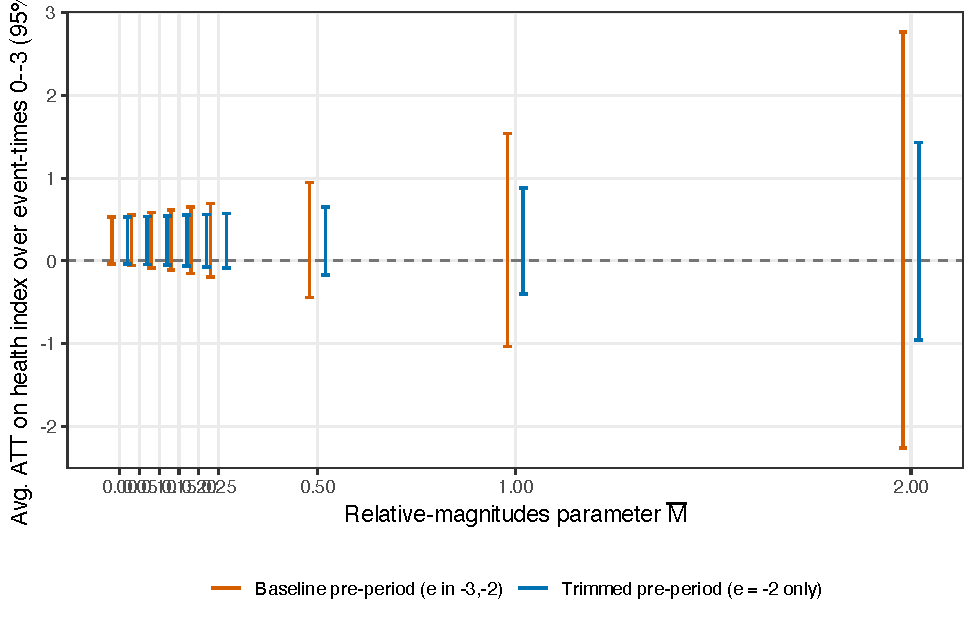
\includegraphics[width=0.92\textwidth]{figures/honestdid_joint_sensitivity.pdf} \caption{PTA-sensitivity bounds on the CS estimate of the average health-index ATT over event-times 0--3. Vermilion bars are the baseline pre-period specification (e $\in \{-3, -2\}$); blue bars are the trimmed pre-period specification (e = $-2$ only). The baseline CI widens quickly with $\bar{M}$; the trimmed CI widens slowly.} \label{fig:honestdid} \end{figure}

The original CS interval already includes zero ($[-0.036,\, 0.532]$), consistent with the marginal 10\%-level significance reported in Section~\ref{sec:results}, and the robust interval at $\bar{M} = 0$ is essentially identical under both specifications. At $\bar{M} = 0.25$ the two diverge substantially: the baseline robust CI widens to $[-0.194,\, 0.694]$, while the trimmed robust CI widens only to $[-0.090,\, 0.572]$. At $\bar{M} = 1$ the gap is wider still: $[-1.036,\, 1.541]$ under baseline versus $[-0.403,\, 0.879]$ under the trimmed pre-period.

The gap between the two specifications pinpoints the source of the baseline fragility. The relative-magnitudes restriction bounds admissible post-period drift by the largest pre-period deviation, and the baseline's largest pre-period deviation is the $t=-3$ coefficient of $-0.263$. Under the trimmed pre-period this scale shrinks to $-0.057$, almost a fifth of the baseline, and the robust CI widens much more slowly across the $\bar{M}$ grid. A reader who treats the $t=-3$ spike as a thin-cell extreme-lead noise realisation will find the trimmed specification the more relevant target and will conclude that the CS effect is moderately robust. A reader who treats the $t=-3$ spike as genuine evidence of non-parallel pre-trends will find the baseline specification binding and will conclude that the effect depends on parallel trends holding close to exactly. Both readings are defensible, and the paper reports the sensitivity bounds under both rather than collapsing to a single preferred answer.

\subsection{Alternative cognition outcome}

Table~\ref{tab:child_raven} reports the cognition coefficient using the child Raven score from IFLS Book~EK, which is administered only to respondents aged 7--14 at wave~5. The estimate is essentially zero on a substantially smaller sample, consistent with the null result on the adult IRT-based cognition index in the pooled specification.

\begin{table}[!htbp] \centering \caption{Alternative cognition outcome (child Raven).} \label{tab:child_raven} % Auto-generated by code/R/11_robustness.R
\begin{tabular}{lccc}
\toprule
Outcome & Estimate & SE & N \\
\midrule
Child Raven score & -0.018 & (0.026) & 3,323 \\
\bottomrule
\end{tabular}
 \begin{minipage}{0.85\textwidth} \footnotesize \emph{Notes.} TWFE with community-of-birth and birth-year fixed effects on the child Raven score from IFLS Book~EK, restricted to respondents aged 7--14 at wave~5. Standard errors clustered at the community-of-birth level. \end{minipage} \end{table}
